

%%% This LaTeX source document can be used as the basis for your technical
%%% report. Intentionally stripped and simplified
%%% and commands should be adjusted for your particular paper - title, 
%%% author, citations, equations, etc.
% % Citations/references are in report.bib 

\documentclass[conference,backref=page]{acmsiggraph}
\usepackage{algorithm2e}
\TOGonlineid{45678}
\TOGvolume{0}
\TOGnumber{0}
\TOGarticleDOI{1111111.2222222}
\TOGprojectURL{}
\TOGvideoURL{}
\TOGdataURL{}
\TOGcodeURL{}

% Include this so that citations show up in blue and the page information is included in the reference section
\hypersetup{
    colorlinks = true, 
    linkcolor = blue,
    anchorcolor = red,
    citecolor = blue, 
    filecolor = red, 
}


\title{Travelling Salesman Problem\\
	   Report}

\author{Conner Weatherston \thanks{e-mail:40167111@live.napier.ac.uk} \\
Edinburgh Napier University\\
Algorithms and Data Structures (SET09117)}
\pdfauthor{Conner Weatherston}

\keywords{travelling salesman problem, nearest neighbour, optimisation}

\begin{document}

\teaser{
   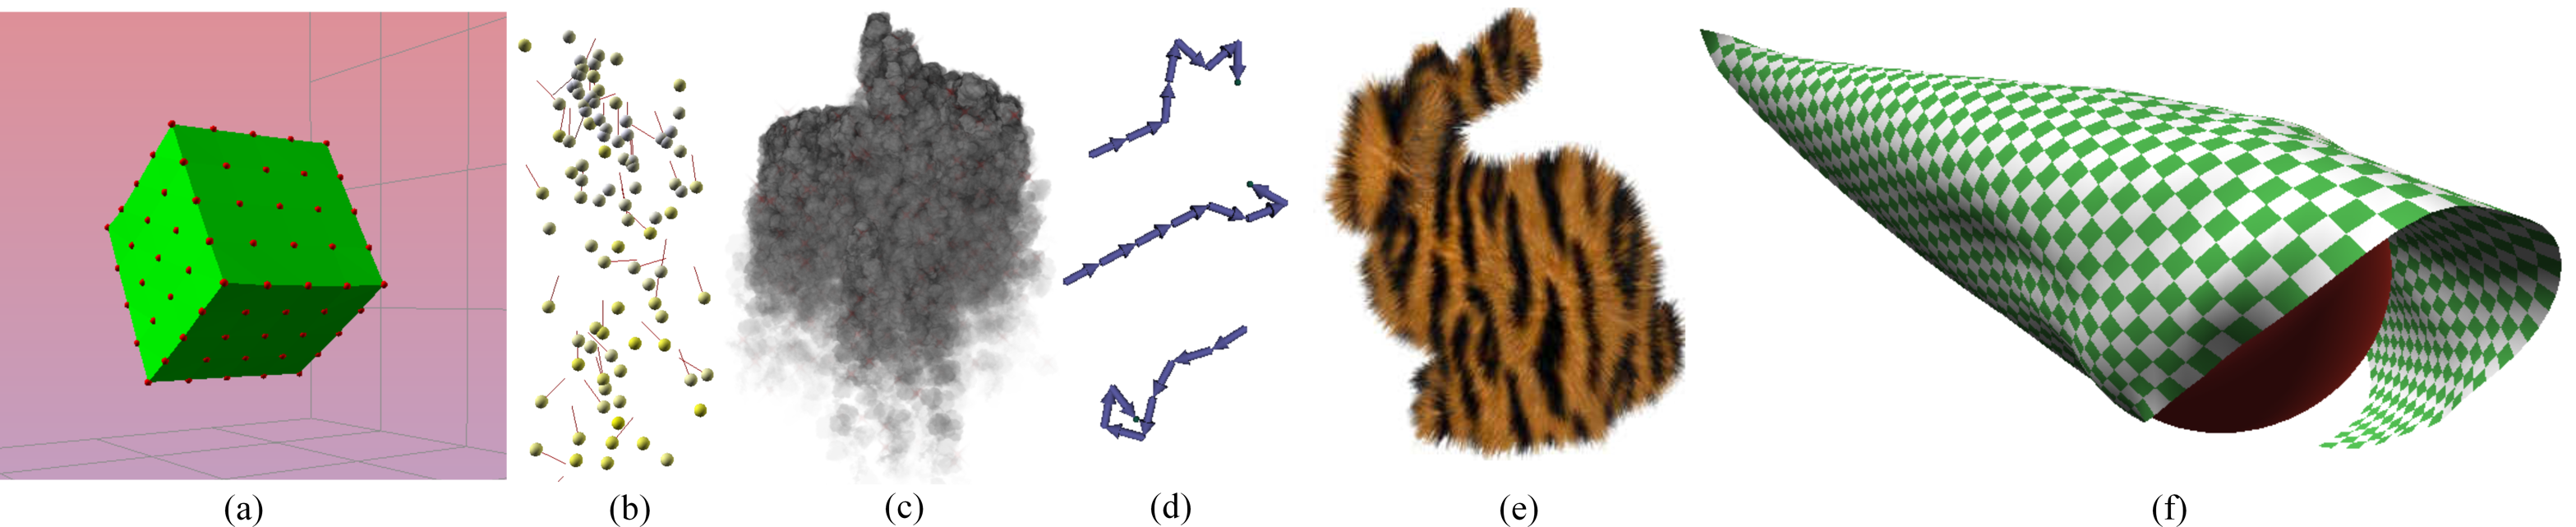
\includegraphics[height=1.5in]{images/sampleteaser}
   \caption{Place a teaser image at the top of your report to show key examples of your work (e.g., multiple screenshots of the different test situations) - Every figure should have a caption and a description.  For example, each figure is labelled and explained: (a) soft bodies, (b) particles, (c) inverse kinematics, (e) fur shells, and (f) position-based dynamics for cloth effects.}
   \label{fig:teaser}
 }

\maketitle

\raggedbottom

\begin{abstract}

PLACE ABSTRACT HERE.

\end{abstract}



\keywordlist


\section{Introduction}

This report is looking at possible improvements of the nearest neighbour algorithm in order to solve the travelling salesman problem (commonly referred to as tsp). The tsp essentially is a question which asks 'Given a set of cities, what is the shortest route possible that visits each city only once and will return to the origin.

The main issue with the travelling salesman problem is the possible routes available grows exponential with size. In a tsp with 10 cities there is 181,400 possible routes. This is calculated using the formula
 \begin{equation}
P =  \frac{(N-1)!}{2}
\end{equation}
where~$P$ is number of possibilities and~$N$ is number of cities (points).

Only half of the possible routes are counted as each route has an equal reverse route that has the exact same distance. The ~$P$-1 is there since the starting city is defined and the other cities can have different permutations.

\section{Method}
One possible way of computing a tsp is by using the nearest neighbour algorithm. This involves sorting the list so that the next city in the list is the closest city to the current city. 

\underline{Pros}
\begin{itemize}
	\item Easy to implement.
	\item Very quick results for small data sizes.
	\item 
	
\end{itemize}

\underline{Cons}
\begin{itemize}
	\item Requires large storage of data. 
	\item Large searching problems (Have to continually iterate over list until it is empty.)
	\item Assumptions are made about distance (Some routes may be infeasible).
	\item Brute force method.
\end{itemize}

\underline{Pseudocode}


\begin{algorithm}
	\KwData{ArrayList input}
	\KwResult{returns Nearest Neighbour list}
	current city = input first value\
	\While{cities in input}{
		add current city to result\
		distance = max value\
		\ForEach{city in input}
		{
			\If{distance(current city, city) $<$ distance}
			{
				closest city = city\
				distance = distance(current point,city)\
			}
		}
		remove closest city from input\
		current city = closest city\
	}
\caption{Nearest neighbour algorithm}
\end{algorithm}



A variation to the nearest neighbour algorithm is comparing the distance along an axis. In theory this should give a quicker computation time as it is only comparing two numbers and avoids using any squaring and square rooting.

As it is based on the nearest neighbour still there is very little difference in the algorithm. 

\begin{algorithm}
	\KwData{ArrayList input}
	\KwResult{returns Nearest Neighbour list}
	current city = input first value\
	\While{cities in input}{
		add current city to result\
		closest x = max value\
		\ForEach{city in input}
		{
			\If{city.x $<$ current city.x}
			{
				closest city = city\
				closest x = city.x\
			}
		}
		remove closest city from input\
		current city = closest city\
	}
	\caption{Nearest x neighbour algorithm}
\end{algorithm}

\begin{algorithm}
	\KwData{ArrayList input}
	\KwResult{returns Nearest Neighbour list}
	current city = input first value\
	\While{cities in input}{
		add current city to result\
		closest y = max value\
		\ForEach{city in input}
		{
			\If{city.y $<$ current city.y}
			{
				closest city = city\
				closest y = city.y\
			}
		}
		remove closest city from input\
		current city = closest city\
	}
	\caption{Nearest y neighbour algorithm}
\end{algorithm}

\section{Results}
\paragraph{Data set rl5915}\hfill


rl5915 has a size of 5915 and when unsorted has a total distance of 1.0145047117318021E7.
 \\  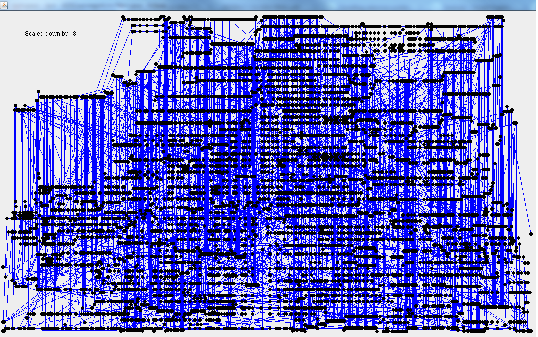
\includegraphics[height=1.5in]{images/rl5915unsorted}


\begin{center}	
	
		Nearest Neighbour

	\begin{tabular}{| l | l | l | l |}
		\hline
		Attempt & Total Distance (m) & Time Taken (ms)\\ \hline
		1 & 707498.63 & 207 \\ \hline
		2 & 707498.63 & 188  \\ \hline
		3 & 707498.63 & 185 \\ \hline
		4 & 707498.63 & 186 \\ \hline
		5 & 707498.63 & 185 \\ \hline
		Average & 707498.63 & 190 \\ \hline
	\end{tabular}
	
   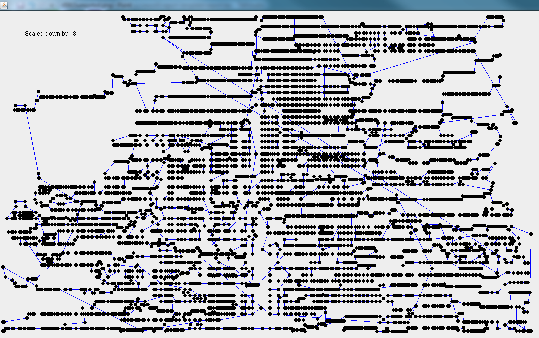
\includegraphics[height=1.5in]{images/rl5915nn}
\end{center}


\begin{center}	
	
	Nearest X Neighbour
	
	\begin{tabular}{| l | l | l | l |}
		\hline
		Attempt & Total Distance & Time Taken\\ \hline
		1 & 11C & 22C \\ \hline
		2 & 9C & 19C  \\ \hline
		3 & 10C & 21C \\ \hline
		4 & 10C & 21C \\ \hline
		5 & 10C & 21C \\ \hline
		6 & 10C & 21C \\ \hline
		Average & 10C & 21C \\ \hline	
	\end{tabular}
	
	IMAGE FOR SORTED ROUTE GOES HERE.
\end{center}


\begin{center}	
	
	Nearest Y Neighbour
	
	\begin{tabular}{| l | l | l | l |}
		\hline
		Attempt & Total Distance & Time Taken\\ \hline
		1 & 7787705.43 & 98 \\ \hline
		2 & 7787705.43 & 80  \\ \hline
		3 & 7787705.43 & 76 \\ \hline
		4 & 7787705.43 & 77 \\ \hline
		5 & 7787705.43 & 76 \\ \hline
		Average & 7787705.43 & 81 \\ \hline
	\end{tabular}
	
	 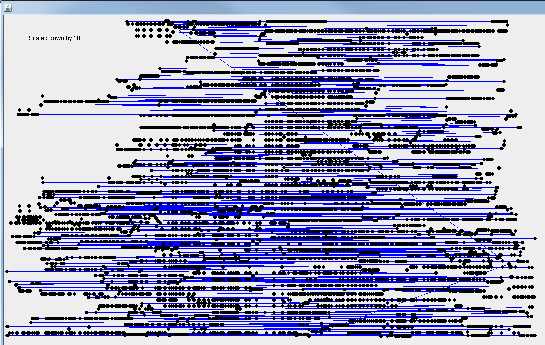
\includegraphics[height=1.5in]{images/rl5915ny}
\end{center}






Due to the nature of the nearest neighbour algorithm some of the variations implemented would only result in a difference in time taken to compute the algorithm. However it is possible to compare the nearest neighbour with nearest x and nearest y as they produce different routes. 

 WHAT WAS THE FASTEST/ SLOWEST / BEST RESULT/ WORST RESULT FOR SMALLEST 
 
 
 WHAT WAS THE FASTEST/ SLOWEST / BEST RESULT/ WORST RESULT FOR LARGEST
 
 
 WHAT WAS THE FASTEST/ SLOWEST / BEST RESULT/ WORST RESULT FOR AVERAGE
 
 WHAT WAS SURPRISING.
 
 WHAT IMPROVEMENTS CAN BE MADE.
  

\section{Conclusion and Future work}
The report should finish with a summary to give a brief overview of what the reader should remember most.  What was most important? The future work part only needs to be covered in your final report.


% \section*{Acknowledgements}


\bibliographystyle{acmsiggraph}
\bibliography{report}

\end{document}

